\begin{center}
    \begin{adjustbox}{max totalsize = {\textwidth}{\textheight}}
        \forestset{
            path highlight/.style = {
                draw = red,
                line width = 10mm, 
                edge = {<-, red, line width = 5mm},
                for ancestors = {
                    draw = red,
                    line width = 5mm, 
                    edge = {<-, red, line width = 5mm}
                }
            },
            same state/.style = {
                draw = red,
                line width = 15mm
            }
        }
        % from https://tex.stackexchange.com/questions/493991/beamer-and-forest-dynamically-highlight-a-path-from-the-root-to-a-node-in-a-t
        \forestset{alt/.code args={<#1>#2#3}{%
            \alt<#1>{\pgfkeysalso{for tree={#2}}}{\pgfkeysalso{for tree={#3}}}},
            onslide/.code args={<#1>#2}{%
            \only<#1>{\pgfkeysalso{for tree={#2}}} 
        }}

        \begin{forest}
            for tree = {
                l sep = 10em,
                edge = {line width = 5mm, ->},
            }
             [{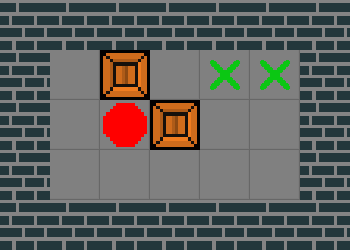
\includegraphics{search_tree/1.png}},
                [{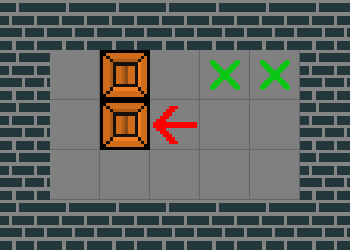
\includegraphics{search_tree/1_1.png}}
                    [{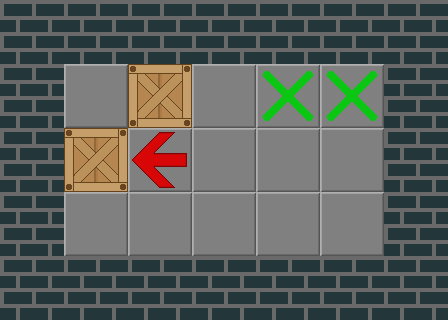
\includegraphics{search_tree/1_1_1.png}}
                        [{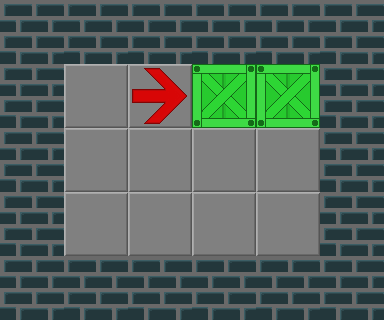
\includegraphics{search_tree/1_1_1_1.png}}]
                        [{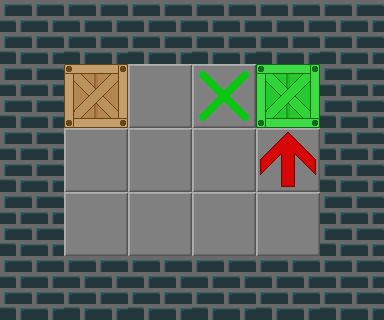
\includegraphics{search_tree/1_1_1_2.png}}, onslide=<3>{same state}]
                    ]
                    [{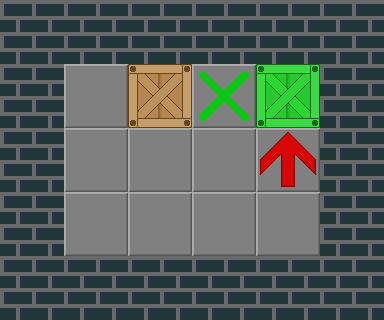
\includegraphics{search_tree/1_1_2.png}}
                        [{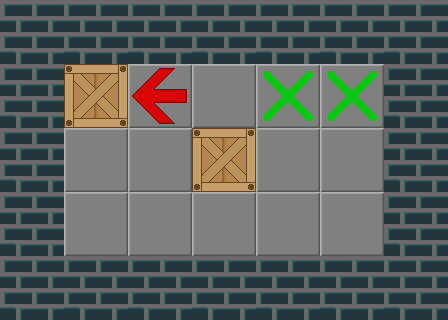
\includegraphics{search_tree/1_1_2_1.png}}, onslide=<2>{path highlight}]
                        [{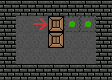
\includegraphics{search_tree/1_1_2_2.png}}, onslide=<3>{same state}]
                    ]
                ]
                [{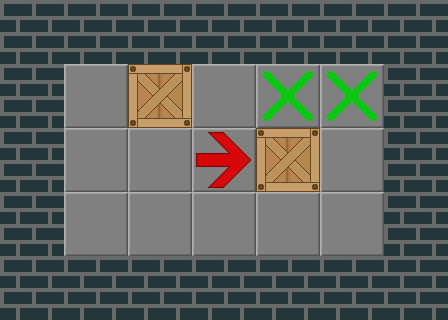
\includegraphics{search_tree/1_2.png}}, onslide=<3>{same state}
                    [{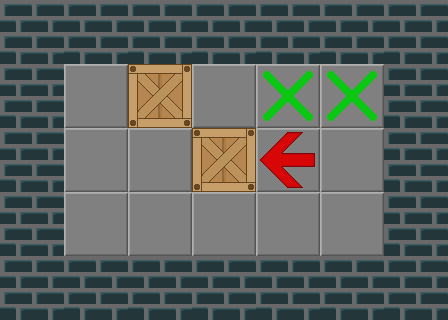
\includegraphics{search_tree/1_2_1.png}}, onslide=<3>{style={draw = none, inner sep = 0, line width = 0}}
                        [{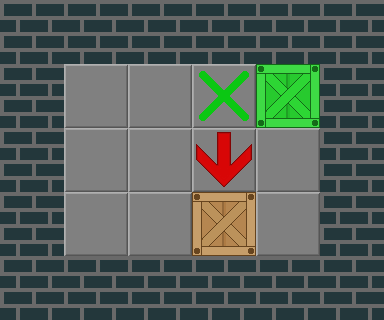
\includegraphics{search_tree/1_2_1_1.png}}, onslide=<3>{style={draw = none, inner sep = 0, line width = 0}}]
                        [{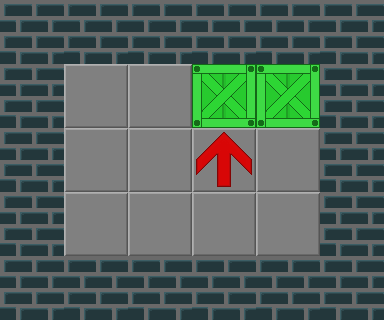
\includegraphics{search_tree/1_2_1_2.png}}, onslide=<3>{style={draw = none, inner sep = 0, line width = 0}}]
                    ]
                    [{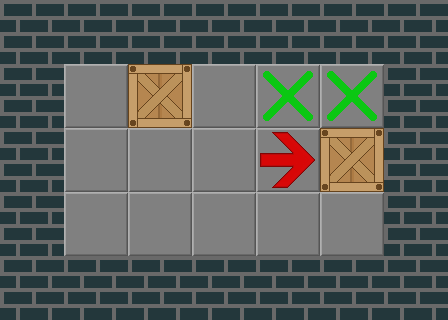
\includegraphics{search_tree/1_2_2.png}}, onslide=<3>{style={draw = none, inner sep = 0, line width = 0}}
                        [{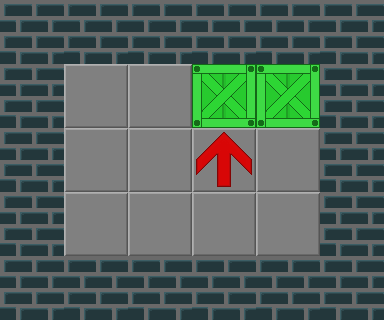
\includegraphics{search_tree/1_2_2_1.png}}, onslide=<3>{style={draw = none, inner sep = 0, line width = 0}}]
                        [{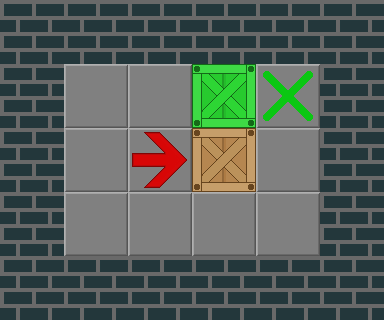
\includegraphics{search_tree/1_2_2_2.png}}, onslide=<3>{same state}]
                    ]
                ]
            ]
        \end{forest}
    \end{adjustbox}
\end{center}